In this section we try to find a model able to explain the variable ``PTS'' through regression techniques.

First of all a preliminary analysis was performed on the data to get some intuitive insights about their composition and relations.
\Fig~\ref{fig:CorrMatrix} shows the correlation matrix over the entire dataset.
\begin{figure}[H]
	\centering
	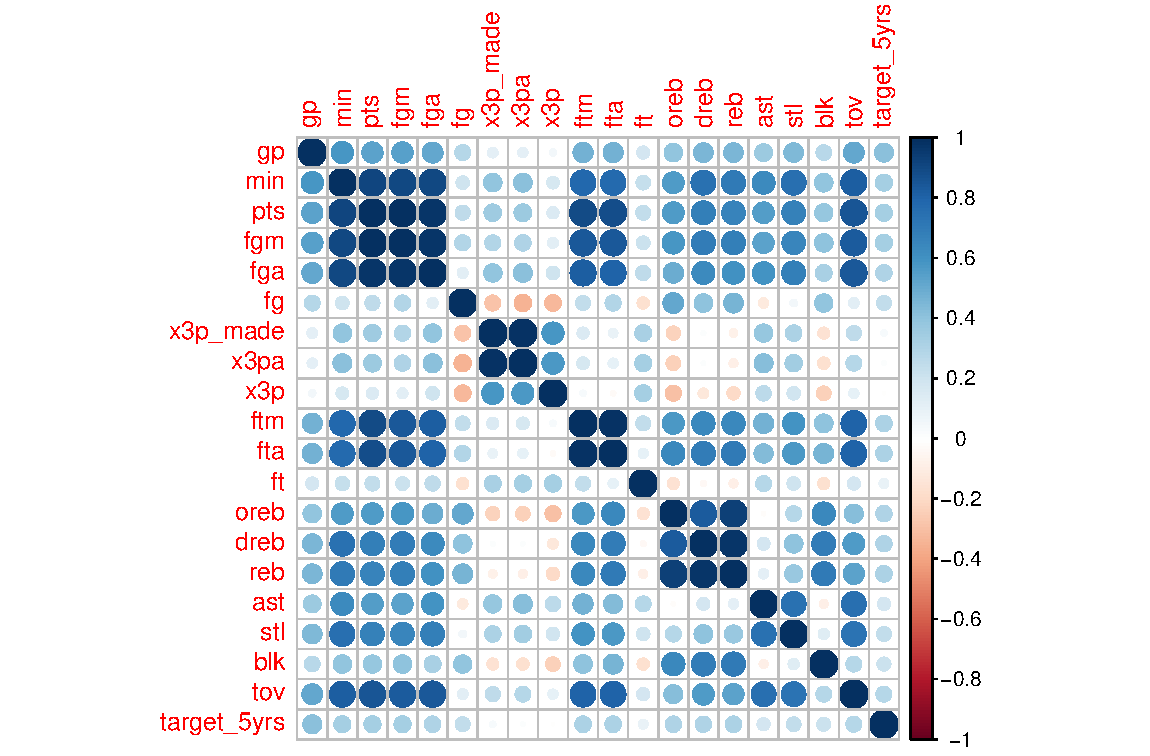
\includegraphics[width=0.75\linewidth]{ImageFiles/Regression/CorrMatrix.pdf}
	\caption{Correlation matrix.}
	\label{fig:CorrMatrix}
\end{figure}

From that matrix it is possible to see that ``PTS'' is strongly correlated with ``MIN''. Intuitively players who play more time have more chances to gain points, and players who make more points will be put on the game for more time by the coach. Therefore this result is consistent with the intuition.
The other two variables strongly correlated are ``FGM'' and ``FGA'', but for different reasons. Actually ``FGM'' tells the number of field goals made, which serves as the main source of points. Indeed, by fitting a linear model using only ``FGM'' as regressor, we obtained a model with $R^2 = 0.9815$. Similarly for ``FGA'' since it is the total amount of field goals attempts. With this remark in mind, we decided to exclude both of these variables from our analysis because they are almost equivalent to the target and they are not interesting for our analytical purposes.

After this overview, subset selection and regularization methods were applied to select the variables to include in the linear model. More precisely, the methods used were:
\begin{itemize}
	\item Forward stepwise selection;
	\item Backward stepwise selection;
	\item Ridge regression;
	\item Lasso regression.
\end{itemize}
